\begin{figure*}[t]
  \title{Accuracy at Various Hidden Unit/Layer Combinations}
\centering
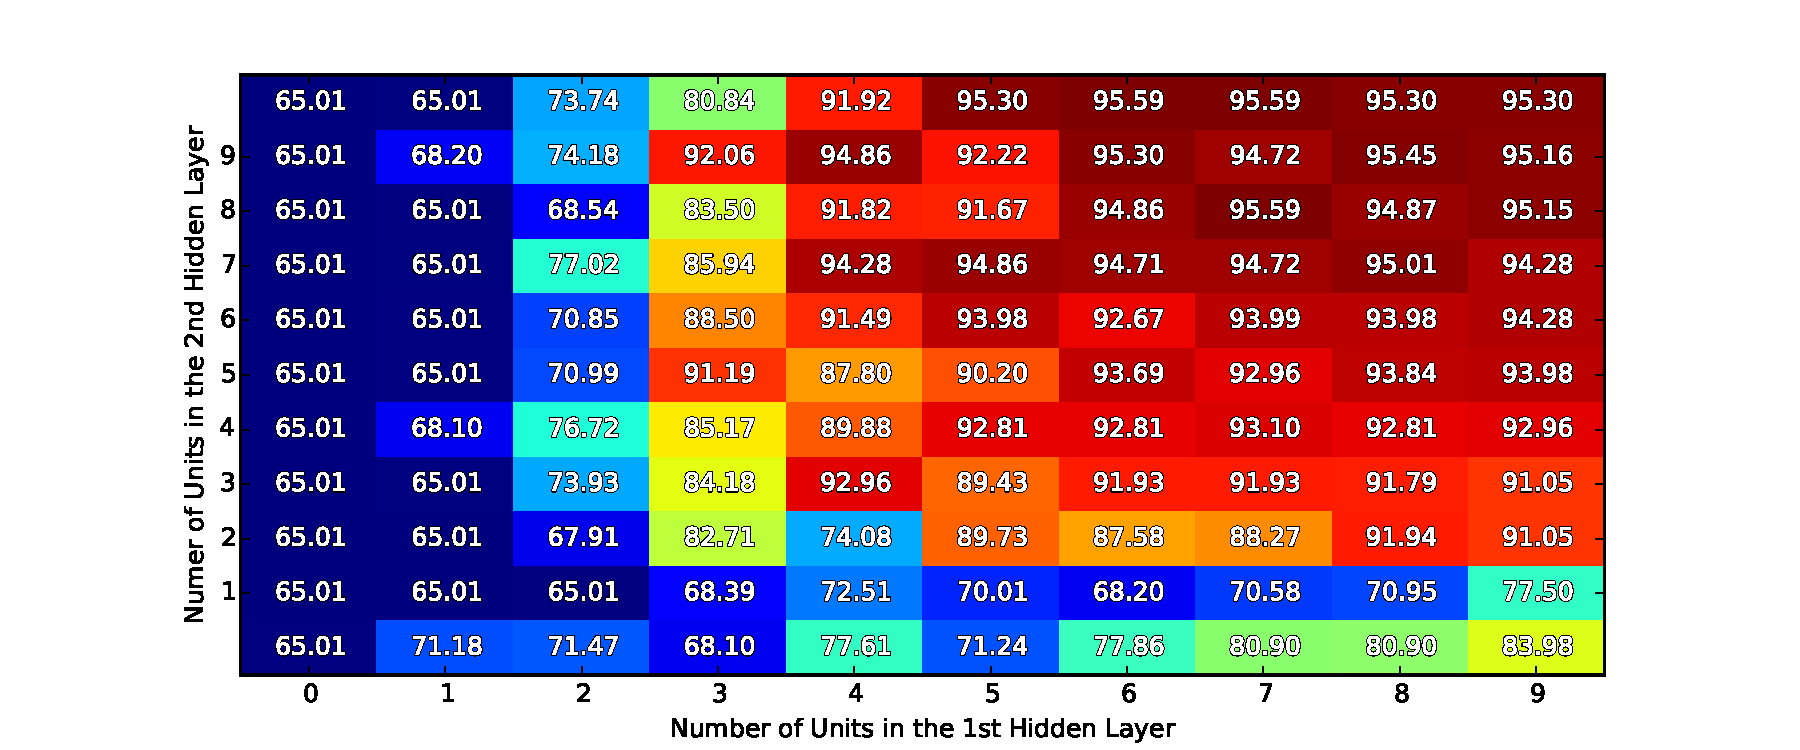
\includegraphics[width=\textwidth]{figs/wbcd_table}
\caption {Accuracy for neural networks with one and two hidden layers. Entry \(i,j\) represents a neural network with \(j\) units in the first hidden layer and \(i\) units in the second hidden layer ({\em i.e.,} row 0 represents neural networks with only one hidden layer). The bold entry represents max accuracy.}
\label{fig:wbcd_table}

\end{figure*}


\begin{figure}[t]

\centering
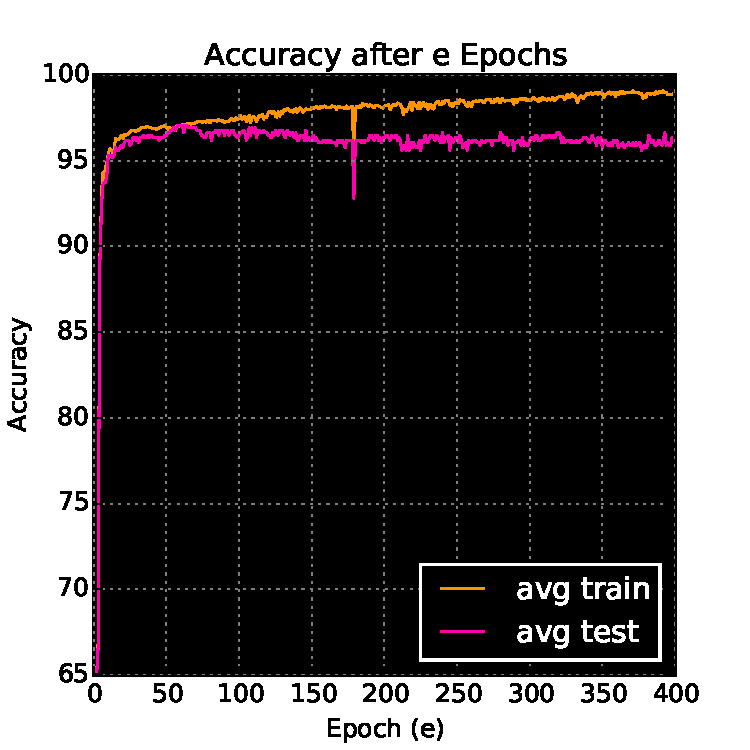
\includegraphics[width=0.95\columnwidth]{figs/wbcd_iterative}
\caption {The figure shows the average accuracy on the training and test sets at every epoch from 1 to 400 for a neural network with 8 units at the first hidden layer and 8 units at the second. TODO: add fold talk}
\label{fig:wbcd_iterative}

\end{figure}


\begin{figure}[t]

\centering
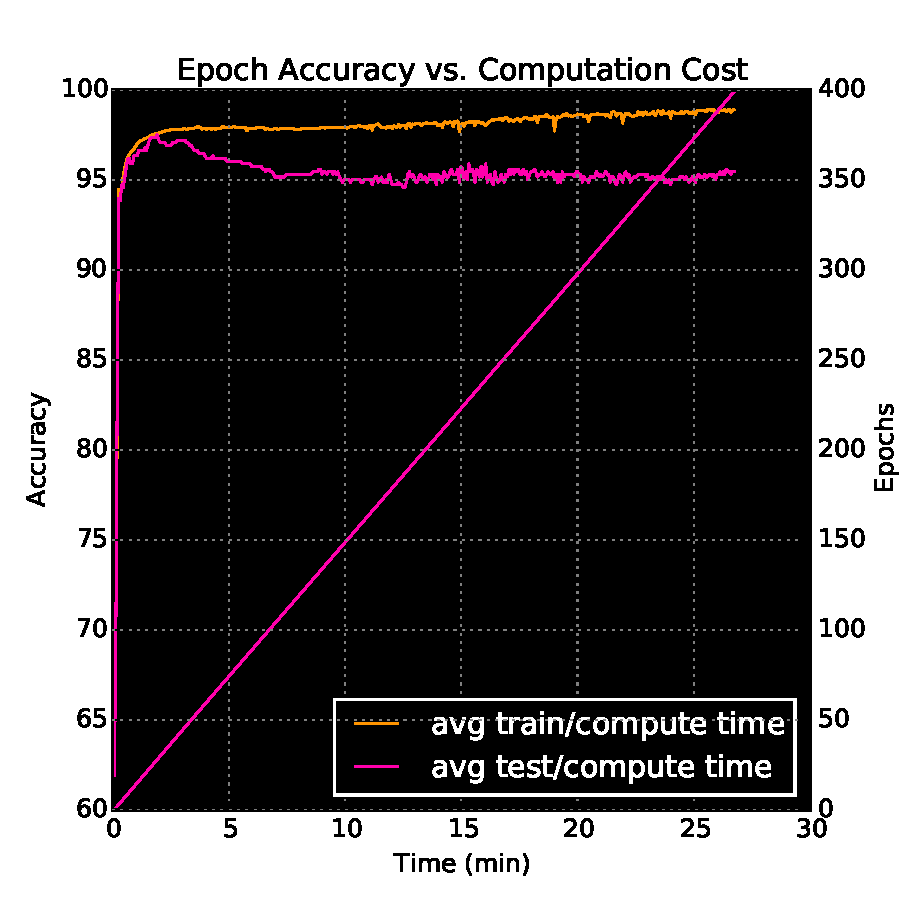
\includegraphics[width=0.95\columnwidth]{figs/wbcd_timing_iterative}
\caption {Add caption}
\label{fig:wbcd_iterative_timing}

\end{figure}


\begin{figure}[t]

\centering
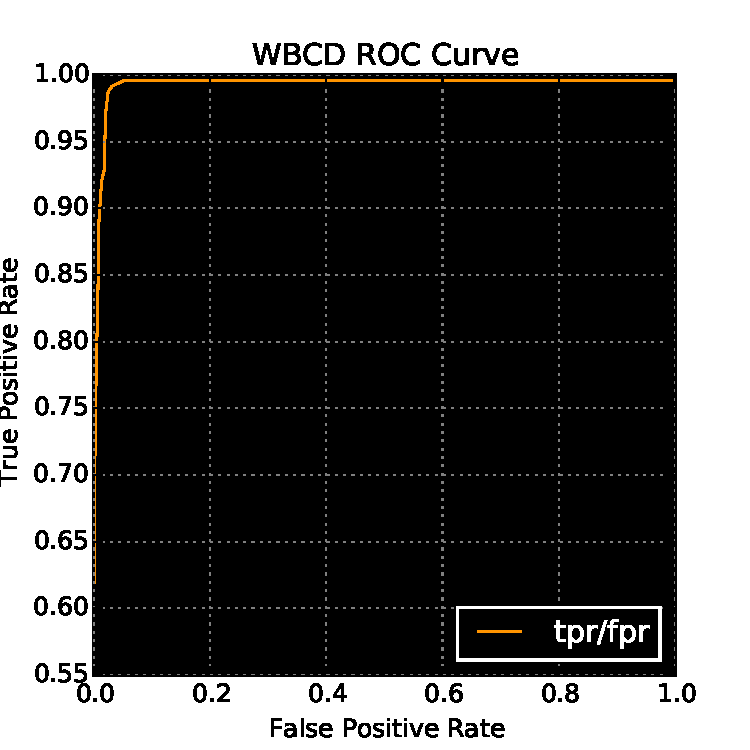
\includegraphics[width=0.95\columnwidth]{figs/wbcd_roc}
\caption {Add caption}
\label{fig:wbcd_roc}

\end{figure}


\begin{figure}[t]

\centering
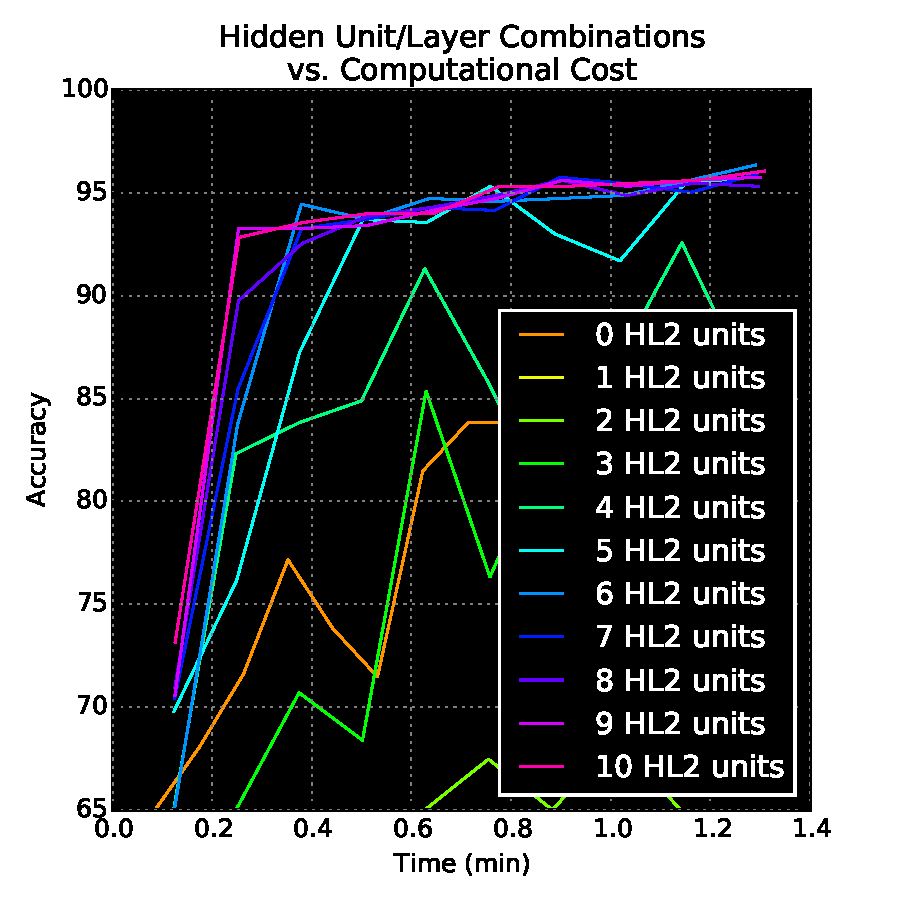
\includegraphics[width=0.95\columnwidth]{figs/wbcd_timing}
\caption {Add caption}
\label{fig:wbcd_timing}

\end{figure}

RESULT CHECKLIST:\\
1. Add the ensemble plot\\
2. Discuss each plot in turn (interesting point from each)\\
3. Synthesize general result message (prediction accuracy vs. cost)\\
